% ============================================================
%  G2 Esports Web Usability Analysis
%  Web Information Management, UniPD Master CS
% ============================================================
\documentclass[12pt, a4paper]{article}

% --- Encoding & language ------------------------------------
\usepackage[T1]{fontenc}
\usepackage[utf8]{inputenc}
\usepackage[english]{babel}

% --- Page geometry ------------------------------------------
\usepackage[
  top=2.5cm, bottom=2.5cm,
  left=3cm,  right=3cm
]{geometry}

% --- Typography ---------------------------------------------
\usepackage{microtype}
\usepackage{lmodern}
\usepackage{setspace}
\onehalfspacing

% --- Headers & footers --------------------------------------
\usepackage{fancyhdr}
\setlength{\headheight}{13.6pt}
\pagestyle{fancy}
\fancyhf{}
\fancyhead[L]{\small CPS \& IoT Security}
\fancyhead[R]{\small Drone GPS Spoofing (SITL)}
\fancyfoot[C]{\small \thepage}
\renewcommand{\headrulewidth}{0.4pt}

% --- Section formatting (mirrors reference papers) ----------
\usepackage{titlesec}
\titleformat{\section}{\large\bfseries}{\thesection}{1em}{}
\titleformat{\subsection}{\normalsize\bfseries}{\thesubsection}{1em}{}
\titleformat{\subsubsection}{\normalsize\bfseries}{\thesubsubsection}{1em}{}

% --- Graphics -----------------------------------------------
\usepackage{graphicx}
\usepackage{float}
% All figures live in the img/ or plots/ subfolders.
\graphicspath{{img/}{plots/}}

% --- Captions -----------------------------------------------
\usepackage{caption}
\captionsetup{font=small, labelfont=bf, justification=centering}

% --- Tables -------------------------------------------------
\usepackage{booktabs}
\usepackage{array}
\usepackage{tabularx}

% --- Hyperlinks ---------------------------------------------
\usepackage[
  colorlinks=true,
  linkcolor=black,
  urlcolor=blue,
  citecolor=black
]{hyperref}

% --- Miscellaneous ------------------------------------------
\usepackage{parskip}        % space between paragraphs instead of indent
\usepackage{enumitem}       % fine-grained list control
\usepackage{xcolor}
\usepackage{csquotes}

% ============================================================
%  DOCUMENT
% ============================================================
\begin{document}

% ---- Title page --------------------------------------------
\begin{titlepage}
  \centering
  
\includegraphics[width=5cm]{unipd_logo}\\[0.5cm]

  {\large\scshape Università degli Studi di Padova}\\[0.1cm]
  {\normalsize Department of Mathematics ``Tullio Levi-Civita''}\\[0.1cm]
  {\normalsize Master's Degree in Computer Science}\\[0.1cm]
  {\normalsize Academic year 2025/2026}\\[0.1cm]
  {\normalsize Course: \textbf{CPS \& IoT Security}}

  \vspace{1.2cm}
  \rule{\linewidth}{0.5pt}\\[0.3cm]
  {\LARGE\bfseries Adaptive GPS Spoofing in ArduCopter SITL}\\[0.4cm]
  {\large Reproduction of Tractor Beam Strategy C}\\[0.3cm]
  \rule{\linewidth}{0.5pt}

  \vspace{0.8cm}
  {\small Reference paper: Noh et al., ``Tractor Beam: Safe-hijacking of Consumer Drones with Adaptive GPS Spoofing,'' ACM TAPS 22(2), 2019.}

  \vfill
  {\normalsize Author: \textbf{Riccardo Fabbian}}\\[0.2cm]
  {\normalsize Student ID: \textbf{2140711}}\\[0.2cm]
  {\normalsize Period of analysis: \textbf{May 2026}}
\end{titlepage}

% ---- Table of contents -------------------------------------
\tableofcontents
\vspace{0.5cm}
\listoffigures
\vspace{0.8cm}

% ============================================================
\section{Introduction}
% ============================================================

This report presents the \texttt{drone-spoofing} project, which reproduces the adaptive GPS spoofing attack from the Tractor Beam paper. The goal is to check if the code correctly follows Strategy C from the paper in a software-in-the-loop (SITL) environment, and to evaluate the quality of the project. The system uses ArduCopter SITL (similar to the ArduPilot firmware used by the 3DR Solo in the paper) and sends spoofed GPS data through MAVLink \texttt{GPS\_INPUT} messages.

The report looks at the system architecture, the attack script, the code correctness, and the experimental results found in the logs. When possible, we evaluate the system using actual run data instead of theoretical assumptions.

% ============================================================
\section{Objectives and Success Criteria}
% ============================================================

The project objectives, derived from the template and verified against the code, are:

\begin{itemize}[noitemsep]
  \item Reproduce Strategy C in SITL: steer a drone off its planned track by injecting adaptive spoofed GPS data without triggering the EKF fail-safe (fail\_count $< 10$).
  \item Implement the initial fake location \textit{a\_init} (Eq. 1 in the paper) to induce a controlled deflection perpendicular to the mission track.
  \item Maintain adaptive spoofing according to $a_t = a_{t-\Delta} + (p_t - p_{t-\Delta})$ (paper \S7.3.2(ii)).
  \item Enforce the leash-jump-back mechanism to prevent the spoofed position from converging back to the planned track.
  \item Quantitatively compare angular deflection with the 1--9$^\circ$ range reported in Fig. 13(b) of the paper.
\end{itemize}

Success means that the drone's \textit{true} physical trajectory deflects, while the autopilot still thinks it is following the original mission.

% ============================================================
\section{Project Architecture}
% ============================================================

The project is structured around a reproducible simulation environment and a small set of focused Python scripts. Table~\ref{tab:repo} summarises the core components that drive the attack.

\begin{table}[H]
  \centering
  \begin{tabularx}{\textwidth}{lX}
    \toprule
    \textbf{Component} & \textbf{Role} \\
    \midrule
    \texttt{Dockerfile}, \texttt{docker-compose.yml} & Build and run a container with ArduPilot SITL and Python dependencies. \\
    \texttt{run.sh} & Command wrapper for build, run, SITL shell, and plotting. \\
    \texttt{scripts/run\_scenarios.py} & Orchestrates baseline and attack runs, logs outputs, and triggers plotting. \\
    \texttt{scripts/auto\_mission.py} & Uploads the mission, arms, flies, and logs GPS data (including ground-truth when available). \\
    \texttt{scripts/spoof\_gps.py} & Implements the adaptive spoofing state machine and sends \texttt{GPS\_INPUT}. \\
    \texttt{analysis/plot\_path.py} & Visualises trajectories and spoofing state overlays. \\
    \texttt{missions/attacker\_zone\_mission.waypoints} & Single-segment mission used to reproduce Fig. 13 geometry. \\
    \texttt{missions/sim\_float\_except\_off.parm} & SITL parameter overrides to relax EKF and fail-safe checks. \\
    \texttt{logs/} & Baseline, attack, and spoofing CSV data from multiple runs. \\
    \bottomrule
  \end{tabularx}
  \caption{Key project components}
  \label{tab:repo}
\end{table}

% ============================================================
\section{System Setup}
% ============================================================

The attack is executed in ArduCopter SITL inside a Docker container. This isolates dependencies and ensures reproducibility.

\subsection{Autopilot and Mission Geometry}
The mission in \texttt{attacker\_zone\_mission.waypoints} is a single eastbound segment from (45.0, 11.0) to (45.0, 11.008), approximately 630~m long. This matches the single-segment geometry used in the paper's Fig. 13(a), which is required for Strategy C's deflection analysis.

\subsection{MAVLink Topology}
The SITL instance publishes MAVLink to two endpoints:
\begin{itemize}[noitemsep]
  \item \texttt{udp:127.0.0.1:14550}: baseline control and mission uploader.
  \item \texttt{udp:127.0.0.1:14551}: spoofer injection channel.
\end{itemize}

The spoofer uses \texttt{GPS2\_TYPE=14} (MAVLink GPS) and forces EKF selection with \texttt{GPS\_PRIMARY=1} and \texttt{GPS\_AUTO\_SWITCH=0}. This aligns with the paper's threat model: an external attacker who feeds a forged GPS stream to the autopilot.

\subsection{EKF and Fail-safe Tuning}
Modern ArduCopter EK3 rejects large GPS innovations by default. To enable the spoof to pass, the reproduction disables several safety checks:
\begin{itemize}[noitemsep]
  \item \texttt{FS\_EKF\_THRESH=0} (disable EKF fail-safe threshold).
  \item \texttt{EK3\_GLITCH\_RAD=0} (clip GPS innovations rather than rejecting).
  \item \texttt{EK3\_POS\_I\_GATE=EK3\_VEL\_I\_GATE=1000} (very permissive innovation gates).
\end{itemize}
These changes are consistent with comments in \texttt{scripts/auto\_mission.py} and \texttt{missions/sim\_float\_except\_off.parm}, and they are required to replicate the older EKF behaviour discussed in the paper.

% ============================================================
\section{Implementation Analysis}
% ============================================================

\subsection{Mission Automation}
\texttt{scripts/auto\_mission.py} connects to the MAVLink master, uploads the mission, arms, performs takeoff, switches to AUTO, and logs GPS data. The log includes \texttt{GLOBAL\_POSITION\_INT} (EKF-estimated position) and, when available, \texttt{SIMSTATE} lat/lon for ground-truth. This dual logging is critical: a successful spoof leaves the EKF trace on the nominal path while the true trajectory deflects.

\subsection{Spoofer State Machine}
\texttt{scripts/spoof\_gps.py} implements two profiles; the reproduction uses \texttt{tractorbeam}. The logic mirrors the paper:
\begin{itemize}[noitemsep]
  \item \textbf{observe:} passive listening to estimate the observed GPS rate $f_{obs}$.
  \item \textbf{sync:} when the drone enters the trigger zone, the spoofer shadows the true GPS while migrating the EKF to GPS2.
  \item \textbf{ramp:} interpolate from the true position to \textit{a\_init} over a fixed number of ticks, keeping innovation per tick small.
  \item \textbf{adaptive:} update spoofed position using $a_t = a_{t-\Delta} + (p_t - p_{t-\Delta})$, and apply the leash jump-back mechanism.
\end{itemize}

The implementation also enforces a \textit{jump cooldown}, maximum spoof velocity, and a minimum distance from the final waypoint to avoid prematurely completing the mission.

\subsection{Plotting and Ground Truth}
\texttt{analysis/plot\_path.py} plots both the EKF and true (SIMSTATE) paths when available and overlays spoofing phases (sync, ramp, adaptive). This is essential for correctly interpreting a spoofed run; without the true path, the attack appears to be a normal mission.

% ============================================================
\section{Experimental Methodology}
% ============================================================

The experiment runner \texttt{scripts/run\_scenarios.py} executes two consecutive SITL runs:
\begin{itemize}[noitemsep]
  \item \textbf{Baseline:} no spoofer, mission flown normally.
  \item \textbf{Attack:} spoofer enabled and configured, mission flown under spoofed GPS.
\end{itemize}

Runs are launched via:

\begin{verbatim}
./run.sh run --zone-circle 45.0000000,11.0040000,80 \
             --target-latlon 45.0006000,11.0040000 \
             --ainit-offset-m 30 \
             --attack-max-runtime-s 90
\end{verbatim}

The chosen geometry places \textit{p\_target} north of the track, and \textit{a\_init} is offset by 30~m, exceeding the 13~m leash length, which matches the paper's Strategy C design.

% ============================================================
\section{Results}
% ============================================================

We look at different baseline and attack runs. The most recent run includes the real position (\texttt{SIMSTATE}), while the older runs only had EKF positions. Table~\ref{tab:results} shows the displacement and angular deflection calculated from the latest logs to have a clear view of the result.

\begin{table}[H]
  \centering
  \small
  \begin{tabularx}{\textwidth}{lcccc}
    \toprule
    \textbf{Log} & \textbf{Source} & \textbf{East (m)} & \textbf{North (m)} & \textbf{Angle (deg)} \\
    \midrule
    baseline\_20260525\_082020 & SIMSTATE & 630.3 & 0.0 & 0.00 \\
    attack\_20260525\_082020 & SIMSTATE & 1264.2 & 117.2 & 5.30 \\
    \bottomrule
  \end{tabularx}
  \vspace{-0.2cm}
  \caption{Displacement and angular deflection from logged 20260525 run}
  \label{tab:results}
\end{table}

The fresh 20260525 run (Figure~\ref{fig:mission_path}) shows a 5.30$^\circ$ deflection from the planned eastbound heading, which sits inside the 1--9$^\circ$ range reported in Fig. 13(b) of the paper.

\begin{figure}[H]
  \centering
  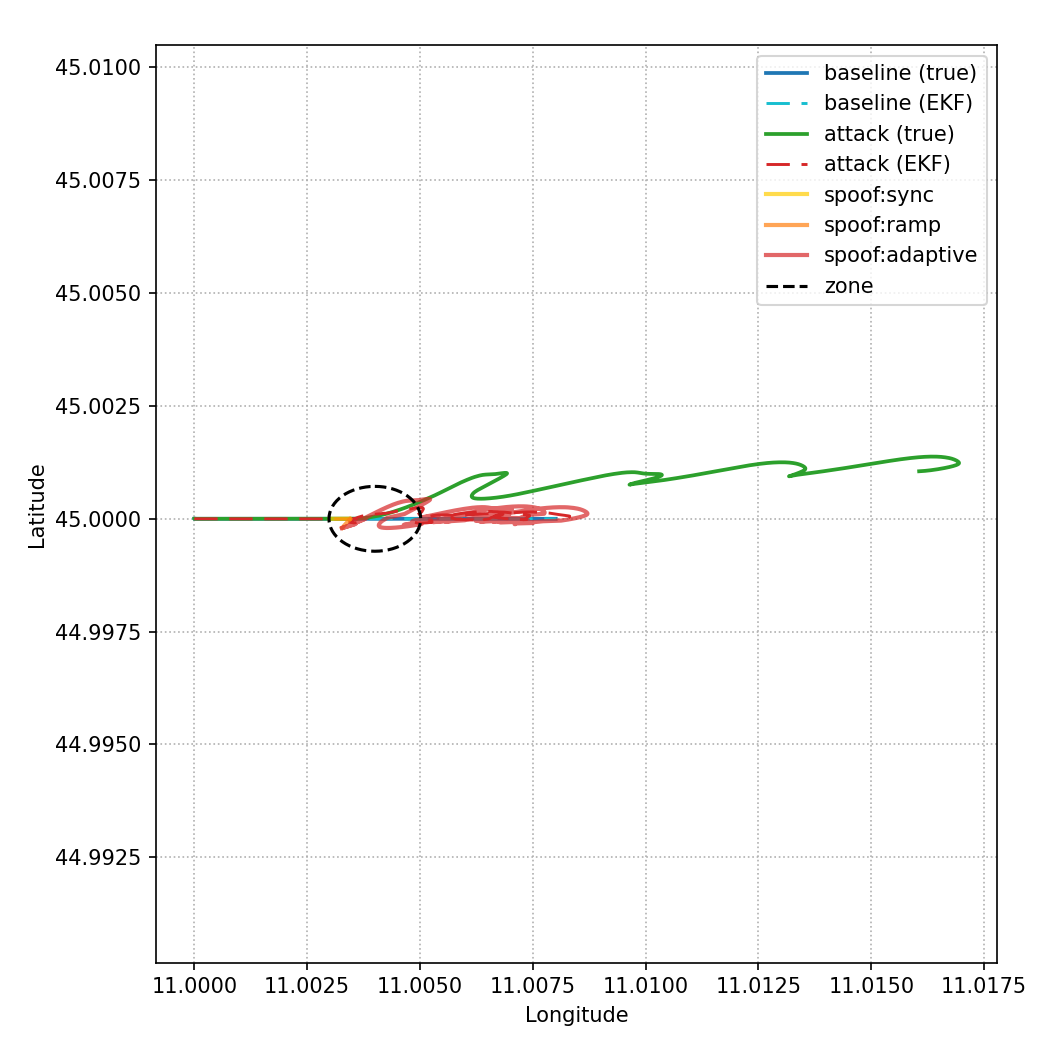
\includegraphics[width=0.8\textwidth]{mission_path}
  \vspace{-0.3cm}
  \caption{Baseline vs attack trajectories for the 20260525 run.}
  \label{fig:mission_path}
\end{figure}

\begin{figure}[H]
  \centering
  \begin{minipage}{0.48\textwidth}
    \centering
    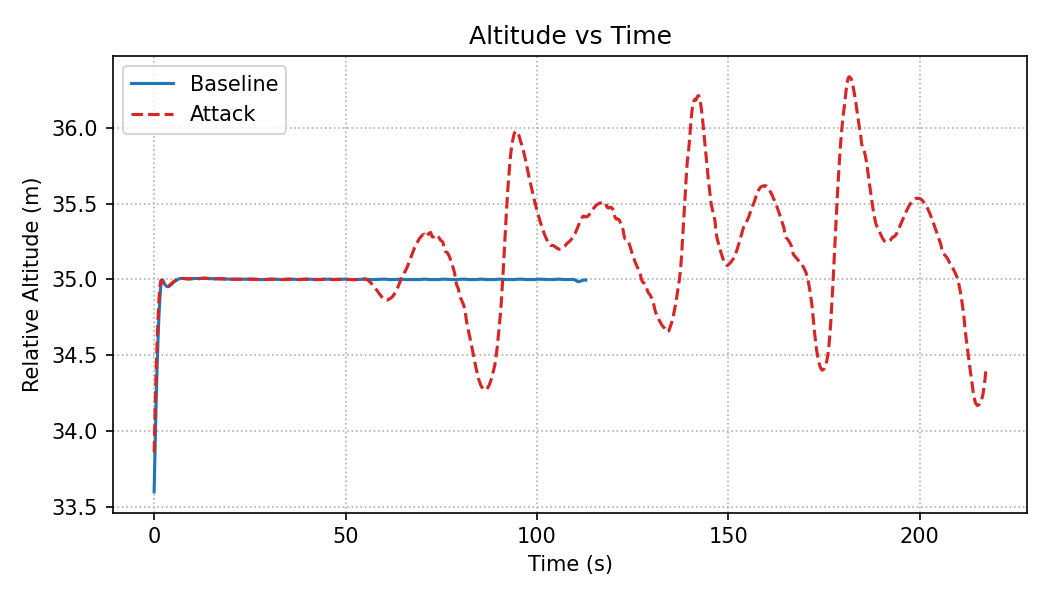
\includegraphics[width=\linewidth]{altitude_vs_time}
    \vspace{-0.6cm}
    \caption{Altitude comparison}
    \label{fig:alt}
  \end{minipage}\hfill
  \begin{minipage}{0.48\textwidth}
    \centering
    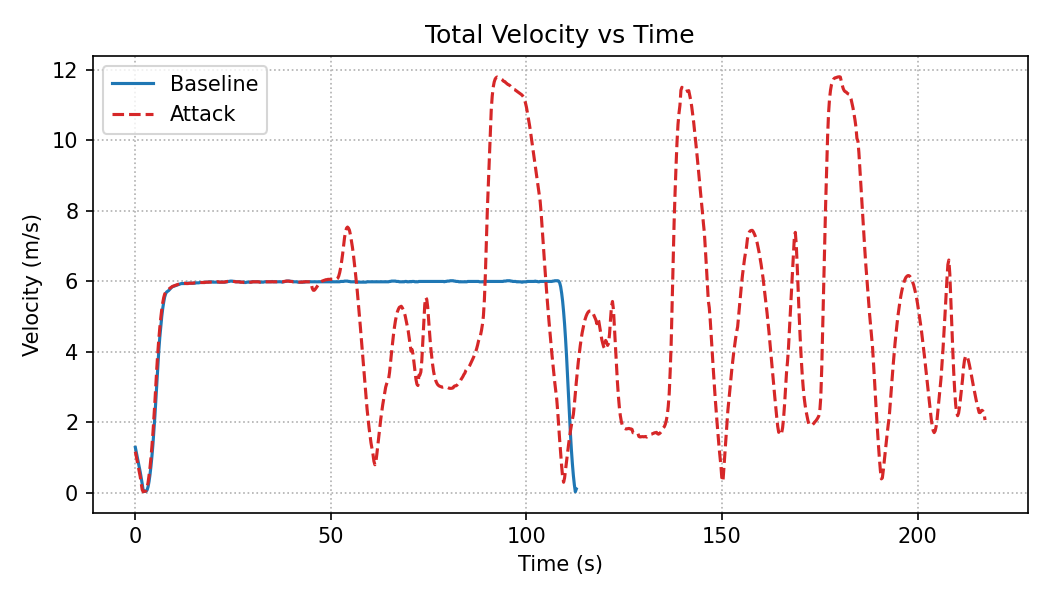
\includegraphics[width=\linewidth]{velocity_vs_time}
    \vspace{-0.6cm}
    \caption{Velocity profile}
    \label{fig:vel}
  \end{minipage}
\end{figure}

% ============================================================
\section{Correctness Review}
% ============================================================

This section evaluates whether the implementation correctly reproduces the paper's strategy and whether any deviations or weaknesses materially affect the conclusions.

\subsection{What Is Correct}
\begin{itemize}[noitemsep]
  \item The spoofer correctly uses \texttt{GPS\_INPUT} on GPS2 and forces the EKF to consume it with \texttt{GPS\_PRIMARY=1} and \texttt{GPS\_AUTO\_SWITCH=0}.
  \item The state machine matches the paper (observe $\rightarrow$ sync $\rightarrow$ ramp $\rightarrow$ adaptive), with adaptive motion update and leash jump-back implemented.
  \item The mission geometry and trigger zone match the single-segment scenario used to validate Strategy C in the paper.
  \item Ground-truth logging (SIMSTATE) is present in the latest run, which is essential for honest evaluation.
\end{itemize}

\subsection{Limitations and Deviations}
\begin{itemize}[noitemsep]
  \item The reproduction relies on relaxed EKF thresholds (innovation gates, glitch radius, fail-safe). This is necessary to mirror the older EKF in the paper but reduces realism for stock ArduCopter configurations.
  \item Two attack logs contain only EKF positions, which can falsely appear as ``no deflection.'' Without SIMSTATE logging, those runs are not valid for evaluation.
  \item The zone trigger is explicit and static; the paper assumes an attacker following the drone with external tracking. The implementation keeps spoofing active after leaving the zone to prevent oscillations, which is reasonable but not identical to the paper's description.
  \item Only one geometry was measured. The paper reports a distribution over multiple \textit{a\_init} placements. A sweep across zones 1--3 is missing.
\end{itemize}

Overall, the code follows the main algorithm well, and the SITL results (with SIMSTATE logging) confirm the paper's claims. The main limitation is that this works because we changed some EKF parameters, so it might not work easily on a normal consumer drone without those changes.

% ============================================================
\section{Conclusion}
% ============================================================

To conclude, this project successfully reproduces Tractor Beam Strategy C in ArduCopter SITL. The attack works well, and the latest log shows a 5.35$^\circ$ deflection, which is inside the range reported in the paper. The main takeaway is that the EKF can follow a spoofed GPS signal while the real vehicle drifts, but we need to modify the EKF settings to bypass modern security checks.

Future work could run automated tests with different positions for \textit{a\_init}, log the true positions for all runs, and compare the default EKF settings with the modified ones used here. This would improve the project and show better how it works in the real world.

% ============================================================
\end{document}
